The requirement that Atmospheric General Circulation Models (AGCMs) exhibit convergent solutions with increasing horizontal resolution was not historically pursued by the community, and as a result many AGCM solutions, such as NCAR's Community Atmosphere Model (CAM), change drastically with resolution. Convergent solutions were likely not pursued during the early AGCM development phase (1950s through the 1980s) due to computational limitations. 

The expanse of computing power beginning around the 1990s permitted convergence tests that indicated AGCMs have weak convergence properties. This issue had largely been ignored, or at least had not become a priority to model developers until recently. Dynamical cores are now more commonly developed with unstructured meshes, which allows for substantial grid flexibility and brining to forefront the issue of convergence. The pursuit of {\em{scale-aware physics}} is in essence an effort to develop closures that result in AGCM solutions to converging with increasing resolution, and that those solutions converge to some reasonable depiction of the atmosphere we live in.

\subsection{Summary}

This work is an effort to understand the specific reasons CAM produces very different solutions with increasing horizontal resolution ---which components of the model are responding to a change in resolution, why is it sensitive to resolution and how does it feedback onto other model components. CAM is an extremely complex model. Understanding why CAM simulates a certain feature a certain way is by no mean trivial. Issac Held authored a paper in 2005 titled {\em{The Gap between Simulation and Understanding in Climate Modeling}} \citep{H2005BAMS}, advocating for the community to shift focus more towards understanding these models. He suggests using a hierarchy of models, from the simplest to the most complex, in order to truly nail down the underlying causes of a phenomenon in an AGCM. This is the approach taken in this thesis.

Chapter~\ref{sec:chapter2} presents the sensitivity of the mean state of CAM, version 4 to horizontal resolutions typical of present-day AGCMs in an aqua-planet configuration. Weak convergence of the mean state is characterized by a progressive drying of the atmosphere and large reductions in cloud coverage with increasing resolution. Analyses of energy and moisture budgets indicate that these trends are balanced by variations in moisture transport by the resolved circulation, and a reduction in activity of the convection scheme. In contrast, the large-scale precipitation rate increases with resolution, which is approximately balanced by greater advection of dry static energy associated with more active resolved vertical motion in the ascent region of the Hadley cell.

An explanation for the sensitivity of the mean state to horizontal resolution is proposed, based on linear Boussinesq theory. The authors hypothesize that an increase in horizontal resolution in the model leads to a reduction in horizontal scale of the diabatic forcing arising from the column physics, facilitating finescale flow and faster resolved convective updrafts within the dynamical core, and steering the coupled system toward a new mean state. This hypothesis attempts to explain the underlying mechanism driving the variations in moisture transport observed in the simulations.

In Chapter~\ref{sec:chapter3}, a set of idealized experiments are developed in CAM to understand the vertical velocity response to reductions in forcing scale that occurs when the horizontal resolution is increased. The test consists of a set of rising bubble experiments, in which the horizontal radius of the bubble and the model grid spacing are simultaneously reduced. The test is performed with moisture, through incorporating moist physics routines of varying complexity, although convection schemes are not considered. Results confirm that the vertical velocity in CAM is to first-order, proportional to the inverse of the horizontal forcing scale, which is consistent with a scale analysis of the dry equations of motion. In contrast, experiments in which the physics time step $\Delta t_{phys}$ are relaxed back to more conventional values results in severely damped vertical motion at high resolution, degrading the scaling. A set of aqua-planet simulations using different physics time steps are found to be consistent with the results of the idealized experiments.

The following two chapters arose from work performed during a year-long visit at NCAR as an Advanced Study Program(ASP) graduate student visitor. Chapter~\ref{sec:chapter4} contains a detailed analysis of the physics-dynamics coupling in CAM's spectral-element dynamical core (CAM-SE), which is uses a continuous Galerkin method, and introduces a new coupling approach. Atmospheric modeling with element-based high-order Galerkin methods presents a unique challenge to the conventional physics-dynamics coupling paradigm, due to the highly irregular distribution of nodes within an element and the distinct numerical characteristics of the Galerkin method. The conventional coupling procedure is to evaluate the physical parameterizations ({\em{physics}}) on the dynamical core grid. Evaluating the physics at the nodal points exacerbates numerical noise from the Galerkin method, enabling and amplifying local extrema at element boundaries. 

Grid imprinting may be substantially reduced through the introduction of an entirely separate, approximately isotropic finite-volume grid for evaluating the physics forcing. Integration of the spectral basis over the control-volumes provides an area average state to the physics, which is more representative of the state in the vicinity of the nodal points rather than the nodal point itself, and is more consistent with the notion of a ``large-scale state'' required by conventional physics packages. This study documents the implementation of a quasi-equal area physics grid into CAM-SE, and is shown to be effective at mitigating grid imprinting in the solution. The physics grid is also appropriate for coupling to other components within the Community Earth System Model, since the coupler requires component fluxes to be defined on a finite-volume grid, and one can be certain that the fluxes on the physics grid are indeed, volume-averaged.

Chapter~\ref{sec:chapter5} describes the implementation of a coarser resolution physics grid into CAM-SE. The dry dynamics is represented by the spectral element dynamical core and tracer transport is computed using the Conservative Semi-Lagrangian Finite Volume Method (CAM-SE-CSLAM). Algorithms are presented that map fields between the dynamics and physics grids while maintaining numerical properties ideal for atmospheric simulations such as mass conservation and mixing ratio shape and linear-correlation preservation. The results of experiments using the lower resolution physics grid are compared to the conventional method in which the physics and dynamical grids coincide. The lower resolution physics grid consists of control volumes designed to provide an isotropic representation of the dynamics to the physical parameterizations, and eliminates grid imprinting, even in regions with steep topography. 

The impact of the coarser resolution physics grid on the resolved scales of motion is analyzed in an aqua-planet configuration, across a range of dynamical core grid resolutions. Through analyzing the relationship between the physics forcing and resolved vertical motion, it was determined that the effective resolution of the model is not degraded through the use of a coarser resolution physics grid. Since the physics makes up about half the computational cost of the conventional CAM-SE-CSLAM configuration, the coarser physics grid may allow for significant cost savings with little to no downside.

Chapter~\ref{sec:chapter6} is the final chapter, and puts together a full picture on the causes of resolutions sensitivity in aqua-planets via a thorough analysis of the CAM-SE-CSLAM simulations from Chapter~\ref{sec:chapter5}. Through scaling the $\Delta t_{phys}$ in the aqua-planets such that the large time-truncation errors discovered in Chapter~\ref{sec:chapter3} may be avoided, it was found that the vertical velocity field everywhere in the model is indeed inversely proportional to the grid spacing of the model. The scaling arises because grid-scale clouds are grid limited; their horizontal extent is set by the effective resolution of the model. The dynamics reacts to grid limited clouds through pressure perturbations of the same scale, and so the pressure gradients, and likewise the vertical velocity both scale in proportion to the inverse of the grid spacing. The scaling indicates that for a doubling of the resolution, the resolved mass flux may be achieved in half the area, which then confines the ascending regions to smaller regions of the model with increasing resolution. To conserve mass, subsiding motion both becomes faster and encompass a larger region in the model with increasing resolution, particularly in the Tropics, which creates a more stable and drier mean state. The tendency towards atmospheric stability with increasing resolution reduces the frequency the deep convection scheme is triggered, and convective precipitation becomes a smaller fraction of the total precipitation rate.

\subsection{Significance and future work}

A solid understanding of the causes of resolution sensitivity in an AGCM is useful in many regards. Many AGCMs now support flexible grid structures, such as variable-resolution grids (VR). VR grids are attractive since they can resolve regional climate processes in a global model, but resolution sensitivity may degrade their value since solutions may be permitted to diverge across the refinement region. To be clear, their are many successful VR studies that do not suffer from the convergence issue, and it is generally safe to use refinement over higher-latitude regions due to relatively subdued buoyancy induced vertical velocities, compared to the tropics. But to completely reconcile this deficiency requires the development of scale-aware physics. Scale-aware physics should be built in part, to anticipate and correct the sensitivity of AGCMs to horizontal resolution, which of course, requires knowledge of the causes of resolution sensitivity.

\begin{figure}[t]
\begin{center}
\noindent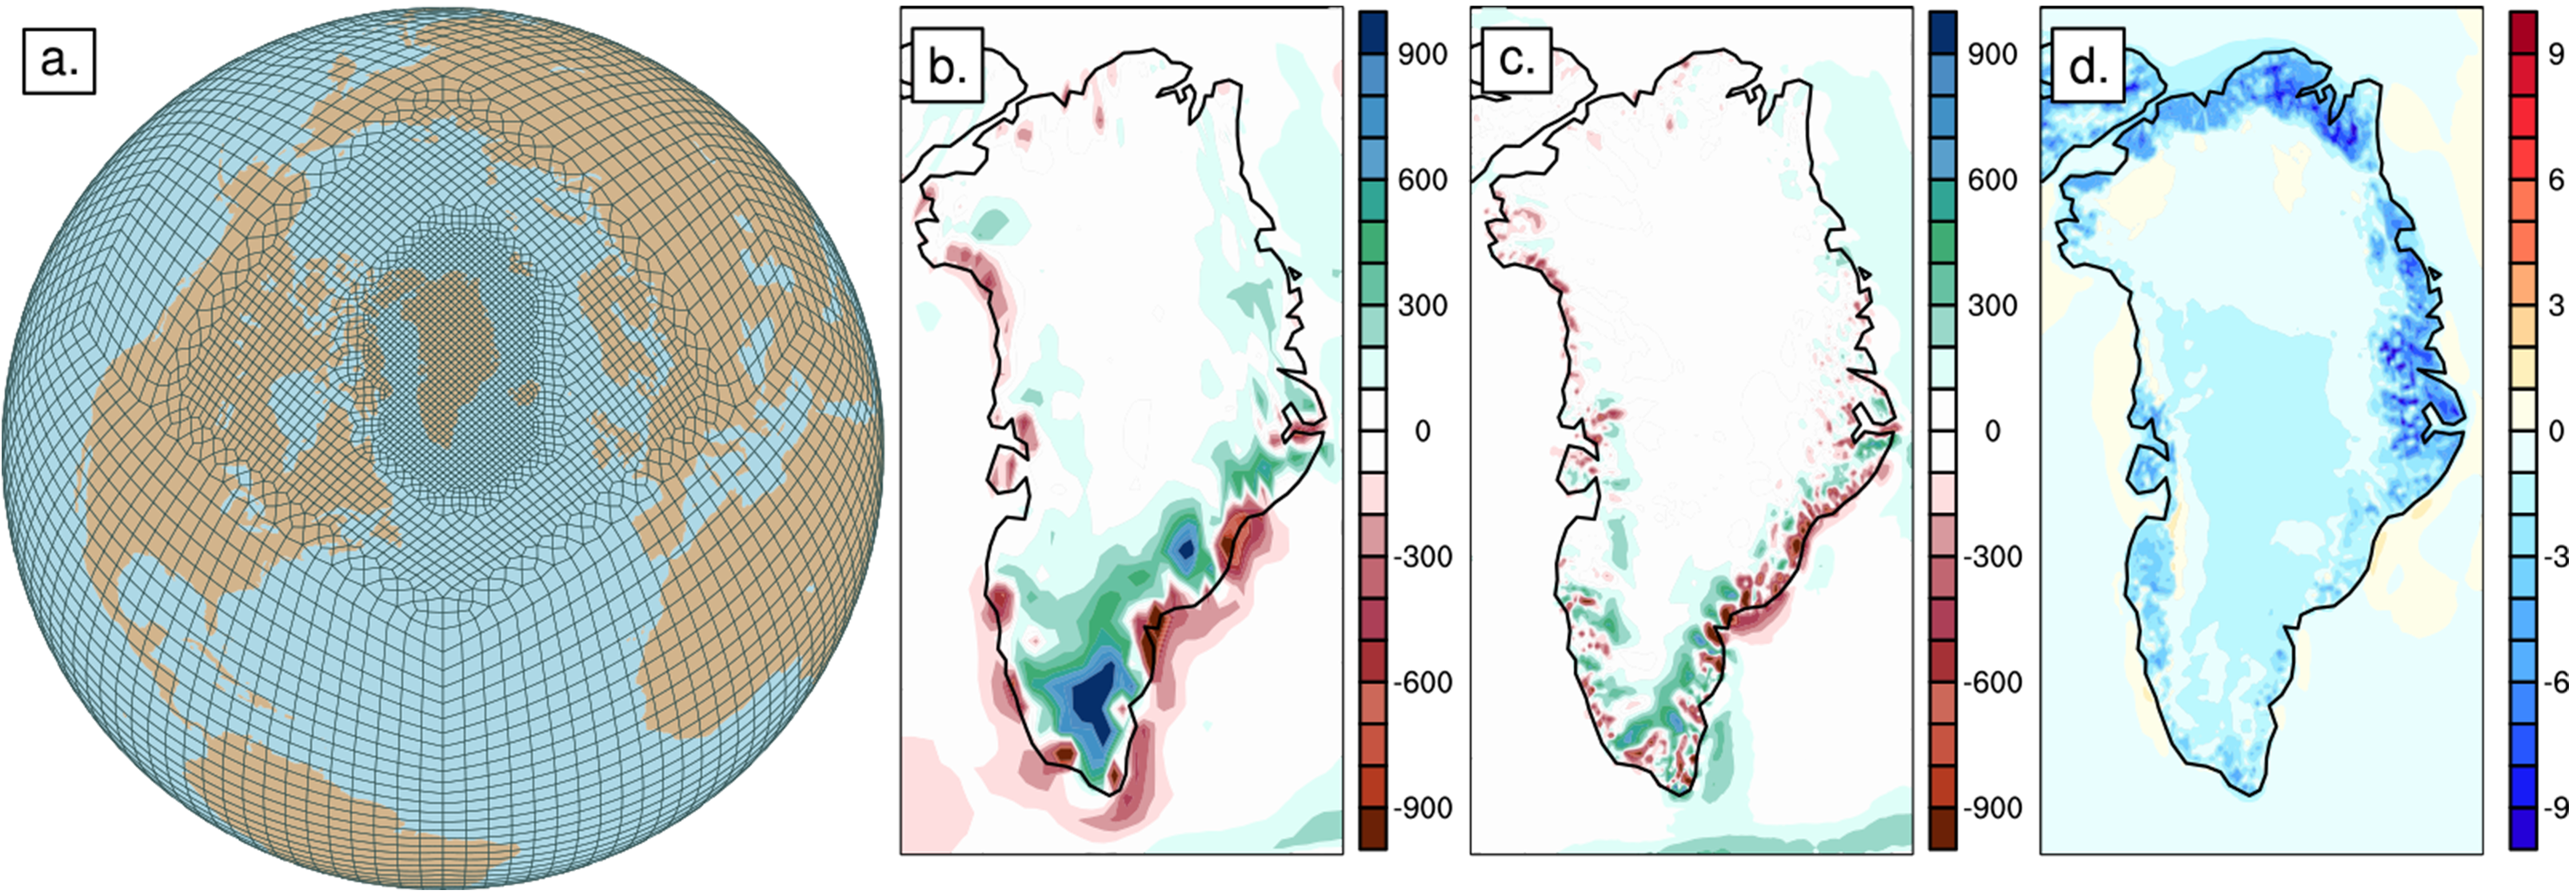
\includegraphics[width=33pc,angle=0]{chapter7/asp_panel.png}\\
\end{center}
\caption{(a.) Variable resolution grid proposed for the pre-industrial control; grid lines delineate the element boundaries of the spectral-element dynamical core, corresponding to an approximate grid spacing of 111.2km in the coarse region and 27.8km in the refined region. CAM-SE $F$ compset simulations using (b.) a uniform 111.2km grid and (c.),(d.) CAM-VR \citep{VETAL2018TC}. Shown are the climatological (1980-1999) (b.),(c.) annually accumulated precipitation difference (mm w.e.) and (d.) JJA 2-meter air temperature difference (K) from the RACMO2 regional climate model simulation.}
\label{fig:se-mesh}
\end{figure}

CAM-SE supports variable resolution grids (CAM-VR), and due to the vast modeling experience that came of this thesis, I was able to assist in a CAM-VR study with regional grid refinement over the big ice sheet in Greenland \citep[Figure~\ref{fig:se-mesh}a;][]{VETAL2018TC}. Recent attempts to couple NCAR's ice sheet model to CAM results in unrealistic ice sheet expansion of the Greenland Ice Sheet due to a high-precipitation bias in southern Greenland, and a summer cold bias on the coastal margins (W. Lipscomb, personal communication). Using CAM-VR, the precipitation bias is successfully improved (Figures~\ref{fig:se-mesh}b,c), indicating the usefulness of the VR approach. Unfortunately, the summer temperature bias remains (Figure~\ref{fig:se-mesh}d). The author has plans to understand and reconcile this bias as an ASP Postdoctoral at NCAR, which would alleviate a major obstacle to realistic simulations of the Greenland Ice Sheet.